%---------------------------------------------------------------------------------------------------
% Einstellungen
% (gelten nur in Zusammenarbeit mit pdflatex)
%---------------------------------------------------------------------------------------------------
\documentclass[
	pagesize,										% flexible Auswahl des Papierformats
	a4paper,											% DIN A4
	oneside,											% einseitiger Druck
	BCOR5mm,											% Bindungskorrektur
	headsepline,										% Strich unter der Kopfzeile
	12pt,											% 12pt Schriftgröße
	halfparskip,										% Europäischer Satz: Abstand zwischen Absätzen
	abstracton,										% Spezielle Formatierung, die erlaubt, dass die
													% Zusammenfassung vor dem Inhaltsverzeichnis steht
	%draft,											% Es handelt sich um eine Vorabversion	
	final,											% Es handelt sich um die endgültige Version
	liststotoc,										% Tabellen- und Abbildungsverzeichnis im Inhaltsverzeichnis
	idxtotoc,										% Index im Inhaltsverzeichnis
	bibtotoc,										% Literaturverzeichnis im Inhaltsverzeichnis
]{book}											% KOMA-Scriptklasse Report


% book hatte ich in der Bachelorarbeit
% article	  <>	 scrartcl
% book	     <>	 scrbook
% report	  <>	 scrreprt
% letter	  <>	 scrlttr2

%-------------------------------------------------------------------------
\usepackage[english,ngerman]{babel}					% deutsche Trennmuster
\addto\captionsngerman{\renewcommand{\figurename}{Abb.}}
\addto\captionsngerman{\renewcommand{\tablename}{Tab.}}
\usepackage[T1]{fontenc}								% EC-Schriften, Trennstellen nach Umlauten
\usepackage[utf8]{inputenc}							% direkte Umlauteingabe (ä statt "a)
													% latin1/latin9 für unixoide Systeme
													% (latin1 ist auch unter Win verwendbar)
													% ansinew für Windows
													% applemac Macs
													% cp850 OS/2

\usepackage{array,ragged2e}							% Wichtig für Abstandsformatierung

%-------------------------------------------------------------------------

% serifenlose Schrift als Standard
% + alle für TeX benötigten mathematischen
%   Schriften einschließlich der AMS-Symbole
%\usepackage{cmbright}						

% skalierte Helvetica als \sfdefault
%\usepackage[scaled=.90]{helvet}				

% Schriften Paket
%\usepackage{times}
% Courier als \ttdefault
\usepackage{courier}

%-------------------------------------------------------------------------
% Anpassung der Kopf- und Fußzeilen
% \usepackage[automark]{scrpage2}
% Korrekter Leerraum nach Befehlsdefinitionen
\usepackage{xspace}
% Dieses Package brauchen wir für den anderthalbzeiligen Abstand.
\usepackage{setspace}
\usepackage[pdftex]{graphicx}
\usepackage[absolute,overlay]{textpos}
\usepackage[final]{pdfpages}

% Neuimplementierung des \cite-Kommandos
\usepackage[numbers, square]{natbib}

% Deutsche Bezeichnungen
\usepackage{bibgerm}		
					
% placing boxes at absolute positions		
\usepackage[absolute]{textpos}	
			
% include pages of external PDF documents	
\usepackage[final]{pdfpages}			
		
% Spaltenbreite bis zur Seitenbreite dehnen	
\usepackage{tabularx}					
		
% Paket zur Erstellung eines Stichwortverzeichnisses
\usepackage{makeidx}				
			
% Automatische Erstellung des Stichwortverzeichnis
\makeindex
\usepackage[intoc, german, prefix]{nomencl}
\makenomenclature

\newcommand{\hyperlinkcolor}{blue}

%-------------------------------------------------------------------------
 \usepackage{graphicx}								% Zur Einbindung von PDF-Bildern
 \usepackage[colorlinks,							% Einstellen und Laden des Hyperref-Pakets
	pdftex,
	bookmarks,
	bookmarksopen=false,
	bookmarksnumbered,
	citecolor=\hyperlinkcolor,
	linkcolor=\hyperlinkcolor,
	urlcolor=\hyperlinkcolor,
	filecolor=\hyperlinkcolor,
	linktocpage,
	pdfstartview=Fit,								% startet mit Ganzseitenanzeige
	pdfsubject={Sprecherlokalisierung unter Verwendung von Mikrofonarrays},
	pdftitle={Masterarbeit im Fachbereich Informations- \& Elektrotechnik an der HAW-Hamburg},
	pdfauthor={Mathias Buder, mathias.buder@gmail.com}]{hyperref}
 \pdfcompresslevel=9
 
%-------------------------------------------------------------------------
% Inhaltsverzeichnis und Abschnittnummerierung
%-------------------------------------------------------------------------
\setcounter{secnumdepth}{2}   % Ich habe recht kurze Kapitel. Die sollen nicht durchnummeriert sein.
\setcounter{tocdepth}{2}

%-------------------------------------------------------------------------% Abbildungsverzeichnis
%-------------------------------------------------------------------------
\graphicspath{{graphics/}}

%-------------------------------------------------------------------------
% Kopf- und Fußzeilen
%-------------------------------------------------------------------------
%\pagestyle{scrheadings}
%\clearscrheadings
%\clearscrplain
%\clearscrheadfoot
%\ohead{\pagemark}
%\ihead{\headmark}

%-------------------------------------------------------------------------
% Neue Befehle
%-------------------------------------------------------------------------
%---------------------------------------------------------------------------------------------------
% Neue Befehle
%---------------------------------------------------------------------------------------------------

%---------------------------------------------------------------------------------------------------
% Umbenennen des Symbolverzeichnisses
%---------------------------------------------------------------------------------------------------
\renewcommand{\nomname}{Glossar}				% Das Symbolverzeichnis heisst nun "Glossar"
\renewcommand{\nomlabel}[1]{					% Die zu erklärenden Begriffe sind nun fett hervorgehoben
	\hfil \textbf{#1} \hfil
}

%---------------------------------------------------------------------------------------------------
% Ein paar ganz nützliche Befehle von Lars Mählmann
%---------------------------------------------------------------------------------------------------
%für Kommentare 
\newcommand{\colb}{\color{green}}
\newcommand{\colbl}{\color{black}}

%---------------------------------------------------------------------------------------------------
% Befehle zum Erstellen des Index
% \addIndexEntry{Eintrag in den Index}
% \addSubIndexEntry{Eintrag in den Index}{Eintrag des übergeordneten Eintrags}
%---------------------------------------------------------------------------------------------------
\newcommand{\addIndexEntry}[1]{#1\index{#1}}
\newcommand{\addSubIndexEntry}[2]{#1\index{#2!#1}}

%--------------------------------------------------------------------------------------------
% LaTeX in eigenem Font
%--------------------------------------------------------------------------------------------
\newcommand{\myLatex}{
	{\rmfamily\LaTeX\xspace}
}

%--------------------------------------------------------------------------------------------
% Befehl zum Erstellen und Hervorheben eines Zitats
% Parameter:
% 1. Zitat
% 2. Author
% 3. Quelle
%--------------------------------------------------------------------------------------------
\newcommand{\myCitation}[3]{
	\begin{flushright}
	\begin{minipage}{.4\linewidth}
		\footnotesize\rmfamily\itshape 
		#1 \\
		\RaggedLeft #2 \\
		#3
	\end{minipage}
	\end{flushright}
	\nobreakspace
}

%--------------------------------------------------------------------------------------------
% Erstellung von Deckblatt (Seite 1) und Titelblatt (Seite 2)
%--------------------------------------------------------------------------------------------
\newcommand{\createCoverAndTitlePage}[7]{
	\createCover{#1}{#2}{#3}{#4}
	\createTitlePage{#1}{#2}{#3}{#4}{#5}{#6}{#7}
}

%--------------------------------------------------------------------------------------------
% Erstellung von Deckblatt (Seite 1) 
% Anwendung:
% \createCover{Art der Arbeit}{Typ der Arbeit}{Autor}{Titel}
%--------------------------------------------------------------------------------------------

\newcommand{\createCover}[4]{

	\thispagestyle{empty}
	\begin{titlepage}

	\setlength{\TPHorizModule}{1mm}
	\setlength{\TPVertModule}{1mm}
	\textblockorigin{0mm}{0mm} % start everything near the top-left corner


	% Art der Arbeit
	\begin{textblock}{111}(83,115)
		\begin{minipage}[c][1,78cm][c]{11,09cm}		
  		\fontsize{24pt}{20pt}
  		\selectfont
  		\begin{center}
  		%\textbf{#1#2} % Bold
  		#1#2
  		\end{center}
		\end{minipage}
	\end{textblock}

	% Name & Titel
	\begin{textblock}{111}(83,131)
		\begin{minipage}[c][4,81cm][t]{11,09cm}	
		\linespread{1.2}	
    		\fontsize{16pt}{14pt}    
    		\selectfont
    		\begin{center}
    			#3 \\ \medskip    
    			#4
    		\end{center}
    		\end{minipage}
	\end{textblock}
	\begin{textblock}{111}(35,260)
		\begin{minipage}[c][1,5cm][t]{7,0cm}		
  		\fontsize{10pt}{10pt}
  		\selectfont
  		\textit{
  		Fakultät Technik und Informatik \\
  		Department Informations- und \\
		Elektrotechnik}
		\end{minipage}
	\end{textblock}


	\begin{textblock}{111}(115,260)
		\begin{minipage}[c][1,5cm][t]{8,0cm}		
  		\fontsize{10pt}{10pt}
  		\selectfont
  		\begin{flushright}
		\textit{
  		Faculty of Engineering and Computer Science \\
  		Department of Information and \\
		Electrical Engineering}
		\end{flushright}
		\end{minipage}
	\end{textblock}

	
%--------------------------------------------------------------------------------------------
% Wichtig! Entsprechendes Auskommentieren!
%--------------------------------------------------------------------------------------------
    
\includepdf{pdf/DeckblattFarbe} 		% zum Ausdruck auf blanko Papier
    %
\includepdf{pdf/titel_leer} 		% zum Ausdruck auf vorgedrucktem papier
    
  % **************************************************************************************
  % Originaldeckblatt mit WORD Vorlage drucken, da nur dort offizieller Schrifttyp vorhanden
  % **************************************************************************************
\end{titlepage}
}

%--------------------------------------------------------------------------------------------
% Erstellung von Titelblatt (Seite 2) 
% Anwendung:
% \createTitlePage{Art der Arbeit}{Typ der Arbeit}{Author}{Titel}{Studiengang}{Erstprüfer}{Zweitprüfer}
%--------------------------------------------------------------------------------------------
\newcommand{\createTitlePage}[8]{
	\thispagestyle{empty}

	\setlength{\TPHorizModule}{1mm}
	\setlength{\TPVertModule}{\TPHorizModule}
	\textblockorigin{0mm}{0mm} % start everything near the top-left corner

	% Name & Titel
	\begin{textblock}{130}(40,63)
		\begin{minipage}[c][5,9cm][t]{13cm}
			\begin{center}
			\linespread{1.2}
			\fontsize{18pt}{18pt}
  		\selectfont
  		#3 \\ \medskip
  		\fontsize{16pt}{16pt}
  		#4
  		\end{center}
		\end{minipage}  	
	\end{textblock}

	% Infos zur Arbeit und zum Deapratment
	\begin{textblock}{126}(32,214)
  	\begin{minipage}[t][6,72cm][l]{12,57cm}
    	\fontsize{12pt}{12pt}
    	\selectfont
    	#1#2 eingereicht im Rahmen der #1prüfung \\
    	im Masterstudiengang #5 \\
			am Department Informations- und Elektrotechnik\\
			der Fakultät Technik und Informatik\\
			der Hochschule für Angewandte Wissenschaften Hamburg\\
			\\\
			Betreuender Prüfer : #6 \\
			Zweitgutachter : #7 \\
			\\\
			Abgegeben am 18. September 2013
  	\end{minipage}
	\end{textblock}
	\	% WICHTIG! Damit wird nach dem Titelblatt eine neue Seite angefangen! Sonst werden Titelblatt &
  	% Danksagung auf eine Seite gedruckt!
}
%--------------------------------------------------------------------------------------------
% Erstellung von Titelblatt (Seite 2) 
% Anwendung:
% \createAbstract{Art der Arbeit}{Typ der Arbeit}{Author}{Titel}{Titel Englisch}{Stichworte}{Keywords}{Zusammenfassung}{Abstract}
%--------------------------------------------------------------------------------------------
\newcommand{\createAbstract}[9]{
	\newpage
	\thispagestyle{empty}

	\subsection*{#3}

	\abstractentry{Thema der #1#2}{#4}
	\abstractentry{Stichworte}{#6}
	\abstractentry{Kurzzusammenfassung}{#8}

	\selectlanguage{english}
	\subsection*{#3}
	\abstractentry{Title of the paper}{#5}
	\abstractentry{Keywords}{#7}
	\abstractentry{Abstract}{#9}
	\selectlanguage{ngerman}
	\
}
%--------------------------------------------------------------------------------------------
% Versicherung über Selbstständigkeit
%--------------------------------------------------------------------------------------------
\newcommand{\asurency}{
	\chapter*{Versicherung über die Selbstständigkeit}
	\vfill
	Hiermit versichere ich, dass ich die vorliegende Arbeit im Sinne der Prü\-fungs\-ord\-nung nach \S 16(5) APSO-TI-BM		ohne fremde Hilfe selbstständig verfasst und nur die angegebenen Hilfsmittel benutzt habe.
Wörtlich oder dem Sinn nach aus anderen Werken entnommene Stellen habe ich unter Angabe der Quellen kenntlich gemacht. 
	\vfill
	\begin{tabularx}{\linewidth}{X l X}
	Hamburg, \today	& \qquad \qquad \qquad	& \\
	\cline{1-1}
	\cline{3-3}
	Ort, Datum	& \qquad \qquad \qquad	& Unterschrift \\
	\end{tabularx}
	\vfill
	\vfill
	\vfill
}

%---------------------------------------------------------------------------------------------------
% Fügt ein Wort dem Index zu
%--------------------------------------------------------------------------------------------
\newcommand{\toIndex}[1]{#1\index{#1}}

%--------------------------------------------------------------------------------------------
% Dient zum Eintragen folgender Dinge in die Zusammenfassung (Abstract):
%	- Thema
% - Stichworte
% - Kurzfassung
% Benutzung wie folgt:
% \abstractentry{Titel}{Text}
%--------------------------------------------------------------------------------------------
\newcommand{\abstractentry}[2]{
	\textbf{\large#1}\\ 
	\nobreakspace 
	\begin{tabular}{lp{142mm}}
		\hspace*{7mm} & #2 \\
	\end{tabular}
	\vfill
}

%--------------------------------------------------------------------------------------------
% Erstellt eine Defintion
% Anwendung: \definition{Die Definition}
%--------------------------------------------------------------------------------------------
\newcommand{\definition}[1]{
\begin{tabular}[ht]{lp{135mm}}
	\textbf{Def.:} & #1 \\
\end{tabular} 
}

%--------------------------------------------------------------------------------------------
% Erstellt eine Widmung
% Anwendung: \dedication{Wem ist das Schriftstück gewidmet}
%--------------------------------------------------------------------------------------------
\newcommand{\createDedication}[1]{
	\newpage
	\thispagestyle{empty}
	\begin{tabular}{lp{60mm}}
		\hspace*{100mm} & \itshape\rmfamily#1 \\
	\end{tabular}
	\vfill
}

%--------------------------------------------------------------------------------------------
% Häufig verwendete Namen mit Literaturverweis und Indexeintrag
%--------------------------------------------------------------------------------------------
\newcommand{\butrynowski}{Christian Butrynowski\index{Butrynowski, Christian} \citep{Butrynowski:2005}\xspace}
\newcommand{\luepke}{André Lüpke\index{Lüpke, André}\citep{Luepke:2004}\xspace}
\newcommand{\bresch}{Marco Bresch\index{Bresch, Marco} \citep{Bresch:2004}\xspace}
\newcommand{\matlab}{MATLAB\textsuperscript{\textregistered}\xspace}
\newcommand{\sennheiser}{Sennheiser\textsuperscript{\textregistered}\xspace}
\newcommand{\ti}{Texas Instruments\textsuperscript{\textregistered}\xspace}
\newcommand{\ccs}{Code Composer\textsuperscript{TM} Studio\xspace}


%---------------------------------------------------------------------------------------------------
% Die folgenden Befehle wurden aus der Vorlage von Michael Knop übernommen
%--------------------------------------------------------------------------------------------
%--------------------------------------------------------------------------------------------
% Ident
%--------------------------------------------------------------------------------------------
\newcommand{\ident}[1]{                             % ein Parameter
	\small\ttfamily#1\sffamily\normalsize
}

%--------------------------------------------------------------------------------------------
% Kürzel
%--------------------------------------------------------------------------------------------
% Hier sind Makros definiert, die die Eingabe erleichtern sollen. Für korrekte Abstände zwischen
% "z.B." sorgt also ein "z.\,B." (LaTeX-Befehl für kleineren Abstand)
% Schneller schreibt sich das durch das Makro "\zB":

% \newcommand{\zB}{z.\,B.\ }

% Hier ist der Rest aber mit dem Paket xspace verwirklicht. Damit kann
% man bei Bedarf den Abstand mit "\hspace" exakt eingeben. Dann zeigt
% LaTeX keine Toleranz bei den Abkürzungen und macht eben exakt das
% untenstehende. 

%\renewcommand{\entryname}{K\"urzel}
%\renewcommand{\descriptionname}{Beschreibung}

\newcommand{\vgl}{vgl.\@\xspace} 
\newcommand{\abb}[1]{Abb.\@\xspace\ref{fig:#1}} 
%\newcommand{\abb}[1]{Abbildung\@\xspace\ref{fig:#1}}
%\newcommand{\abb}[1]{Abbildung\@\xspace\ref{fig:#1} (S.\pageref{fig:#1})}
%\newcommand{\tab}[1]{Tabelle\@\xspace\ref{tab:#1}}
\newcommand{\tab}[1]{Tab.\@\xspace\ref{tab:#1}}
\newcommand{\scr}[1]{Quelltext\@\xspace\ref{lst:#1}} 
\newcommand{\code}[1]{\texttt{#1}} 
\newcommand{\Sec}[1]{Abschnitt\@\xspace \ref{#1}}
\newcommand{\Chap}[1]{Kapitel\@\xspace \ref{chap:#1}} 
\newcommand{\Appx}[1]{Anhang\@\xspace \ref{appx:#1}}  
\newcommand{\Eq}[1]{Gleichung\@\xspace \ref{eq:#1}}  
\newcommand{\zB}{z.\nolinebreak[4]\hspace{0.125em}\nolinebreak[4]B.\@\xspace}
\newcommand{\bzw}{bzw.\@\xspace}
\newcommand{\dahe}{d.\nolinebreak[4]\hspace{0.125em}h.\nolinebreak[4]\@\xspace}
\newcommand{\etc}{etc.\@\xspace}
\newcommand{\bzgl}{bzgl.\@\xspace}
\newcommand{\so}{s.\nolinebreak[4]\hspace{0.125em}\nolinebreak[4]o.\@\xspace}
\newcommand{\iA}{i.\nolinebreak[4]\hspace{0.125em}\nolinebreak[4]A.\@\xspace}
\newcommand{\sa}{s.\nolinebreak[4]\hspace{0.125em}\nolinebreak[4]a.\@\xspace}
\newcommand{\su}{s.\nolinebreak[4]\hspace{0.125em}\nolinebreak[4]u.\@\xspace}
\newcommand{\ua}{u.\nolinebreak[4]\hspace{0.125em}\nolinebreak[4]a.\@\xspace}
\newcommand{\og}{o.\nolinebreak[4]\hspace{0.125em}\nolinebreak[4]g.\@\xspace}

\newcommand{\HAW}{Hochschule für Angewandte Wissenschaften Hamburg\xspace}
\newcommand{\GNU}{GNU\xspace}
\newcommand{\GPL}{\GNU Public License\xspace}

\newcommand{\ACM}{ACM\xspace}
\newcommand{\PDA}{PDA\xspace}
\newcommand{\eqspace}{\hspace{0.5cm}}


%-------------------------------------------------------------------------
% MY COMMANDS
%-------------------------------------------------------------------------
\makeatletter
\long\def\isequal#1#2{\pdf@strcmp{#1}{#2}}
\newcounter{missingfigure}
\newcounter{missingFigureCount} % define counter for missing figures
\newcommand{\size}{1}

\newcommand{\myFigure}[6]{
    \switch
        \case{\isequal{#2}{veryVerySmall}}
            \renewcommand{\size}{0.3\textwidth}
        \case{\isequal{#2}{verySmall}}
            \renewcommand{\size}{0.45\textwidth}
        \case{\isequal{#2}{small}}
            \renewcommand{\size}{0.5\textwidth}
        \case{\isequal{#2}{medium}}
            \renewcommand{\size}{0.65\textwidth}
        \case{\isequal{#2}{big}}
            \renewcommand{\size}{0.8\textwidth}
        \case{\isequal{#2}{Big}}
            \renewcommand{\size}{0.9\textwidth}
        \case{\isequal{#2}{max}}
            \renewcommand{\size}{\textwidth}
    \otherwise
            \begin{center}
                \textbf{\textcolor{red}{FIGURE $\Rightarrow$ No Size Match !!}}
            \end{center}
    \endswitch
    \switch
        \case{\isequal{#1}{missing}}
            \stepcounter{missingFigureCount}
            \begin{figure}[#3]
    		      \begin{center}
			          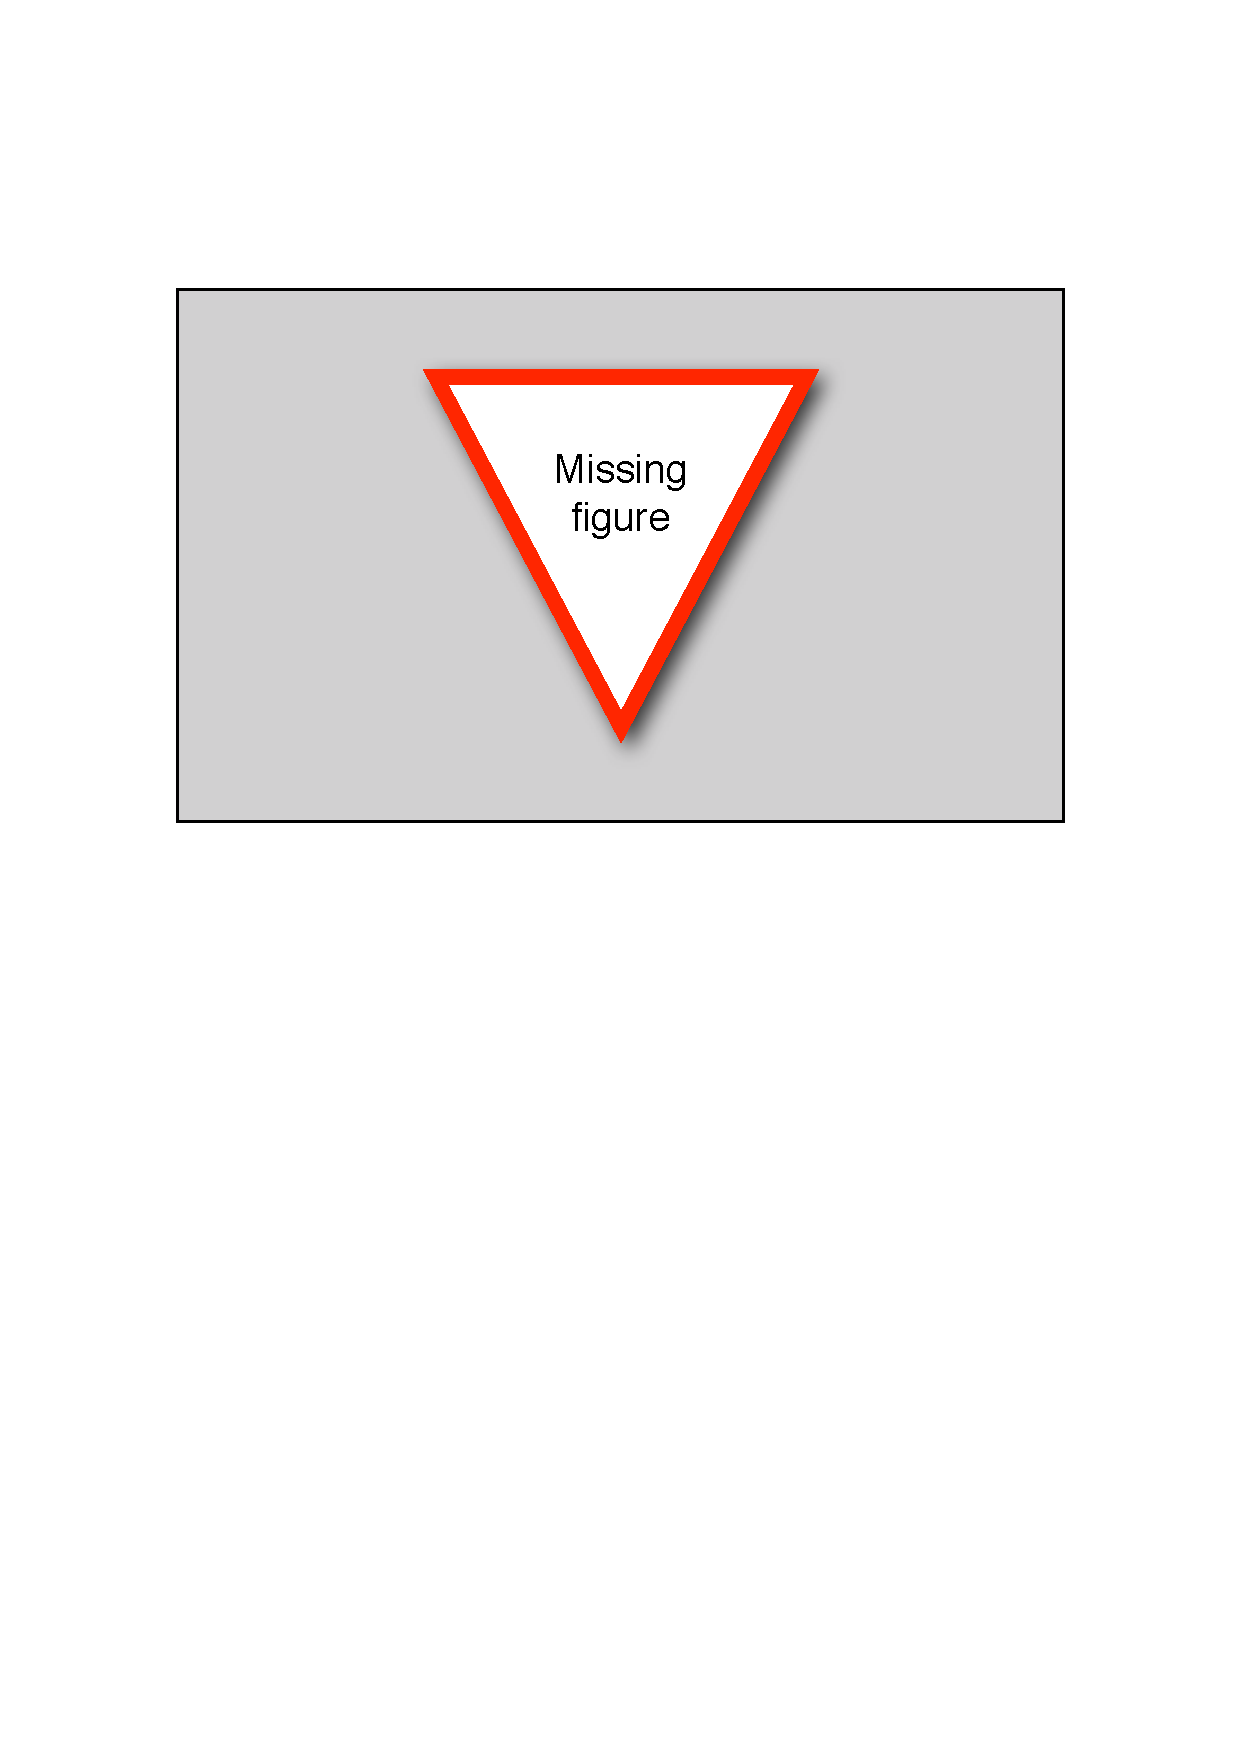
\includegraphics[width=\size]{images/MissingFigure}
			          \caption{\textbf{\textcolor{red}{Missing Figure \themissingFigureCount}} - #4}
			          \label{fig:#5}
		        \end{center}
	        \end{figure}
        \case{\isequal{#1}{real}}
           \begin{figure}[#3]
    		      \begin{center}
			          \includegraphics[width=\size]{images/#6}
			          \caption{#4}
			          \label{fig:#5}
		        \end{center}
	        \end{figure}
        \otherwise
            \begin{center}
                \textbf{\textcolor{red}{FIGURE $\Rightarrow$ No Tag Match !!}}
            \end{center}
    \endswitch
}



%-------------------------------------------------------------------------
% Trennung
%-------------------------------------------------------------------------
%---------------------------------------------------------------------------------------------------
% Trennung
% Hier können alle Wörtertrennungen definiert werden. Die nachfolgenden dienen als Beispiel
% und wurden aus der Vorlage von Michael Knop übernommen.
%---------------------------------------------------------------------------------------------------
\hyphenation{Web-ap-pli-ka-tion Web-ap-pli-ka-tio-nen Web-an-wen-dung Web-an-wen-dung-en My-SQL Kon-text-in-for-ma-ti-onen}

%-------------------------------------------------------------------------
% Anpassung der Parameter, die TeX bei der Berechnung der Zeilenumbrüche verwendet:
%-------------------------------------------------------------------------
\tolerance 1414
\hbadness 1414
\emergencystretch 1.5em
\hfuzz 0.3pt
\widowpenalty=10000
\vfuzz \hfuzz
\raggedbottom


%-------------------------------------------------------------------------
% Meine Pakete:
%-------------------------------------------------------------------------
\setlength {\marginparwidth }{2cm}
\usepackage{todonotes}

\usepackage{caption}
\usepackage{subcaption}
\usepackage{boolexpr,pdftexcmds,trace}
%-------------------------------------------------------------------------
%\usepackage[
    %a4paper,
    %left = 3cm,
    %right = 1.0in,
    %top= 1in,
    %bottom = 0.8in    
%]{geometry}
%\usepackage{showframe} % Show page margin
%-------------------------------------------------------------------------
\usepackage{enumitem}
\usepackage{amsmath}
\usepackage{mathrsfs}
\usepackage{amssymb}
\parindent0pt % do not indet line after new line
\usepackage{trfsigns} % For transformation signs

\usepackage[
    format=hang,
    labelfont=bf,
    textfont=normalfont,
    justification=justified
]{caption}

\usepackage{float} % To force figure position in desired place, use specifier H
\usepackage{cancel}

%-------------------------------------------------------------------------
% Define listing colors
\usepackage{color}
\definecolor{backgroundcolor}{gray}{0.95}
\definecolor{keywordcolor}{cmyk}{0.3,0.76,0,0}
\definecolor{stringcolor}{cmyk}{0.2,0.89,0.97,0.04}
\definecolor{numbergcolor}{cmyk}{0.84,0.64,0,0}
\definecolor{commentgcolor}{cmyk}{0.70,0.14,0.96,0.39}

% Define listing font
% \usepackage[scaled=0.85]{luximono}

% Define listing prperties
\usepackage{listings}
\lstset{
language = C,
numbers=left,
numberstyle=\footnotesize \ttfamily,
stepnumber=1,
numbersep=5pt,
frame=single,                   % adds a frame around the source code
framexleftmargin=8mm,
backgroundcolor=\color{backgroundcolor},
xleftmargin = 0.9cm,
linewidth = \textwidth,
aboveskip = 0.5cm,
%belowskip = 0.5cm,
breaklines = true,
breakatwhitespace = true,
tabsize=2,
basicstyle=\footnotesize \ttfamily,
keywordstyle=\color{keywordcolor}\textbf \ttfamily,
stringstyle=\color{stringcolor}\ttfamily,
commentstyle=\color{commentgcolor}\small \ttfamily,
numberstyle=\tiny,
abovecaptionskip=10pt,
captionpos=b
escapeinside={(*@}{@*)},	% if you want to add a comment within your source code
morekeywords={*,...}     	% if you want to add more keywords to the set
}

\renewcommand{\lstlistlistingname}{Quelltextverzeichnis}
\renewcommand{\lstlistingname}{Quelltext}
%-------------------------------------------------------------------------





